%\documentclass{ExcelAtFIT}
\documentclass[czech]{ExcelAtFIT} % when writing in CZECH
%\documentclass[slovak]{ExcelAtFIT} % when writing in SLOVAK


%--------------------------------------------------------
%--------------------------------------------------------
%	REVIEW vs. FINAL VERSION
%--------------------------------------------------------

%   LEAVE this line commented out for the REVIEW VERSIONS
%   UNCOMMENT this line to get the FINAL VERSION
%\ExcelFinalCopy


%--------------------------------------------------------
%--------------------------------------------------------
%	PDF CUSTOMIZATION
%--------------------------------------------------------

\hypersetup{
	pdftitle={Paper Title},
	pdfauthor={Jan Kadeřábek},
	pdfkeywords={Keyword1, Keyword2, Keyword3}
}


%--------------------------------------------------------
%--------------------------------------------------------
%	ARTICLE INFORMATION
%--------------------------------------------------------

\ExcelYear{2017}

\PaperTitle{Analýza záznamu palubní kamery automobilu}

\Authors{Jan Kadeřábek*}
\affiliation{*%
  \href{mailto:xkader13@fit.vutbr.cz}{xkader13@fit.vutbr.cz},
  \textit{Faculty of Information Technology, Brno University of Technology}}
%%%%--------------------------------------------------------
%%%% in case there are multiple authors, use the following fragment instead
%%%%--------------------------------------------------------
%\Authors{Jindřich Novák*, Janča Dvořáková**}
%\affiliation{*%
%  \href{mailto:xnovak00@stud.fit.vutbr.cz}{xnovak00@stud.fit.vutbr.cz},
%  \textit{Faculty of Information Technology, Brno University of Technology}}
%\affiliation{**%
%  \href{mailto:xdvora00@stud.fit.vutbr.cz}{xdvora00@stud.fit.vutbr.cz},
%  \textit{Faculty of Information Technology, Brno University of Technology}}

\Keywords{Kaskádový klasifikátor --- Mapování dopravního značení --- Palubní kamera}

\Supplementary{\href{https://youtu.be/ywE9Ui8y0Dk}{Demonstrační video} --- \href{https://github.com/jankaderabek/dashcam-analyzer}{GitHub}}


%--------------------------------------------------------
%--------------------------------------------------------
%	ABSTRACT and TEASER
%--------------------------------------------------------

\Abstract{

Podél veřejných komunikací se nachází velký počet dopravního značení. Nikde však nejsou dostupné souhrnné informace  o jeho rozmístění. Vědět, kde je jaká značka je důležité například pro navigační systémy, ale může to být zajímavá informace pro veřejnou správu nebo i běžné občany. Proto se tato práce zabývá analýzou záznamu z palubní kamery, kdy se snaží všechny tyto informace z pořízeného záznamu získat.

Pro popsané účely je využíván kaskádový klasifikátor, který umožňuje rychlou detekci dopravního značení. Následně je využívána klasifikace pomocí k-Nearest Neighbour, která slouží pro klasifikaci typu dopravního značení a případného získání hodnoty na nalezené značce. Práce je implementována v jazyce Python s využitím knihovny OpenCV pro podporu počítačového vidění.

Výsledkem práce je program, který umožňuje zpracovat videozáznam a získat z něj uvedené informace, které lze dále využívat. Detekce dopravního značení dosahuje vysoké spolehlivosti a je tak možné pracovat s reálnými výsledky.

Zpracované informace o dopravním značením je možné snadno vizualizovat na mapě a je možné je zveřejňovat k dalším účelům.
}

\Teaser{
	\TeaserImage{osmdesat.png}
    \TeaserImage{mapa.png}
    \TeaserImage{dvakrat-osmdesat.png}
}



%--------------------------------------------------------
%--------------------------------------------------------
%--------------------------------------------------------
%--------------------------------------------------------
\begin{document}

\startdocument


%--------------------------------------------------------
%--------------------------------------------------------
%	ARTICLE CONTENTS
%--------------------------------------------------------

%--------------------------------------------------------
%--------------------------------------------------------
%--------------------------------------------------------
%--------------------------------------------------------
\section{Úvod}
% * <j.spanhel@gmail.com> 2017-03-29T08:34:22.628Z:
% 
% Jak by měl být strukturovaný úvod říká šablona.
% 
% Další sekce by měli mít následující rozvržení: 
% 2. Related Work
% 3. My solution
% 4. Experiements
% 5. Conclusion
% 
% ^.
Dopravní značení podél veřejných komunikací je velice rozsáhlé a jeho zmapování je vhodné z několika důvodů. Jedná se o užitečné podklady pro navigační systémy a může sloužit také jako informační prostředek pro občany nebo pro městskou správu.

Tato práce si klade za cíl detekovat a rozpoznávat dopravní značení. Za tímto účelem se zabývá detekcí pomocí kaskádového klasifikátoru a rozlišení konkrétních dopravních značek pomocí klasifikace metodou k-Nearest Neighbour. U některých typů dopravních značek následuje klasifikace hodnot v oblasti značky, například při výskytu rychlostního omezení.

V průběhu práce je navrženo řešení, které je schopné implementovat všechny uvedené požadavky. 

Během práce vzniklo několik skriptů v jazyce Python, které postupně zpracovávají jednotlivé kroky celého průběhu analýzy záznamu z palubní kamery.

V úvodní kapitole se nachází analýza existujících řešení a porovnání jejich silných a slabých stránek. V třetí kapitole je popsán celý navržený proces zpracování videozáznamu. Následující kapitola se věnuje postupu implementace jednotlivých částí. V páté kapitole se nachází souhrn provedených experimentů. Na závěr je čtenář informován o vyhodnocené celé práce.


%--------------------------------------------------------
%--------------------------------------------------------
%--------------------------------------------------------
%--------------------------------------------------------
\section{Existující řešení}
\label{sec:HowToUse}
% * <j.spanhel@gmail.com> 2017-04-04T07:31:10.275Z:
% 
% Kaskádový klasifikátor a kNN jsou vaše konkrétní řešení, které jste ve své práci použil.
% To by mělo být až v další sekci (Navrnuté řešení).
% Zde by měl být soupis toho, co jste dosud nastudoval. (Co se dá použít na detekci dopravních značek, co na jejich klasifikaci, rozpoznání atd.)
% 
% ^.
\subsection{Metody detekce dopravního značení}
Základní používanou metodou je detekce v barevném modelu, kdy dochází k extrakci míst do binární reprezentace na základě tolerance pro určitou barvu \cite{color-detection}. Poté se v binární mapě vyhledávají požadované tvary pomocí Houghovy transformace \cite{hough-detection}.

Tyto popsané principy už nejsou příliš moderní, proto se více používá například kaskádový klasifikátor \cite{Viola-Jones}. Ten pracuje na principu posloupnosti několika klasifikátorů za sebou s využitím algoritmu AdaBoost. Jeho výhodou je relativně snadný proces trénování a přesná a rychlá detekce.

Nejpokročilejším způsobem jsou konvoluční neuronové sítě, jejichž aplikace se velmi rozšiřuje \cite{cnn}.



\subsection{Metody klasifikace dopravního značení}

Jednou z možností jak klasifikovat dopravní značení je metoda k-Nearest Neighbour. Ta umožňuje dobře fungující detekci s využitím i menšího množství vzorků \cite{knn}.

Další možností je využít klasifikátory do více tříd (SVM). Jejich využití pro klasifikaci dopravního značení je velmi časté. Základním principem je zde klasifikace příznaků do dvou skupin.

Pro tyto účely je opět možné využít neuronové sítě.


%--------------------------------------------------------
%--------------------------------------------------------
%--------------------------------------------------------
%--------------------------------------------------------
\section{Analýza záznamu}
Proces analýzy záznamu byl rozdělen na několik částí popsaných v následujících kapitolách. Při návrh byl brán potaz na co největší dekompozici problému. Celý proces tedy představuje posloupnost uvedených akcí.

\subsection{Detekce značky}

Prvním bodem analýzy záznamu je detekce samotného dopravního značení. Pro tento účel byl zvolen kaská\-dový klasifikátor jehož princip je popsán v předchozí kapitole. Jeho hlavní výhodou je rychlost detekce, což je důležitý aspekt vzhledem k tomu, že se očekává zpracovávání většího množství dat.

Hlavní skript bude procházet jednotlivé snímky, ve kterých bude hlavním úkolem detektoru nalézt všechny dopravní značky, které se ve snímku nachází. Jedním z požadavků je aby detektor byl schopen nalézt více značek nikoliv jen jednu.

\subsection{Rozlišení typu dopravní značky}

Detekované značky je vhodné klasifikovat podle jejich typu, který vyjadřuje informaci o jakou dopravní značku se jedná. To bude mít na starosti klasifikace pomocí metody k-Nearest Neighbour. Díky tomu, že pomocí detektoru získáme ohraničenou pozici značky bude klasifikace v rámci výřezu poměrně rychlá a spolehlivá.

\subsection{Hodnota dopravní značky}

U některých dopravních značek, zejména u rychlost\-ního omezení, bude zapotřebí dále klasifikovat jejich hodnotu. Tedy v případě značky omezující rychlost získat hodnotu maximální povolené rychlosti v daném místě. 

Pro tuto akci bylo navrhnuto, že se nejprve provede segmentace jednotlivých symbolů, které se nachází v ohraničeném prostoru značky. Symboly pak budou odděleně klasifikovány a následně se sestaví výsledné hodnota.

Klasifikace bude v tomto případě opět probíhat s využitím metody k-Nearest Neighbour \cite{opencv-knn}.


\subsection{Mapování dopravního značení}

Výsledkem procesu analýzy by měl být datový soubor, který bude obsahovat všechny detekované značky a informace o nich jako je typ, případně hodnota a GPS souřadnice s jejich polohou.

Za tímto účelem jsou pořizovány záznamy pomocí mobilní aplikace, které ke každému videozáznamu přiloží soubor obsahující GPS souřadnice v konkrétním čase.

%--------------------------------------------------------
%--------------------------------------------------------



%--------------------------------------------------------
%--------------------------------------------------------



%--------------------------------------------------------
%--------------------------------------------------------
%--------------------------------------------------------
%--------------------------------------------------------
\section{Implementace}
\label{sec:UsefulTools}
Vytvořené řešení využívá metod popsaných v předchozí kapitole. Aby bylo možné využívat jednotlivé metody, bylo nutné připravit datovou sadu pro natrénování použitých algoritmů.

Všechny skripty jsou implementovány v jazyce Python 3 s využitím knihovny pro počítačové vidění OpenCV 3.

\begin{figure}[t!]
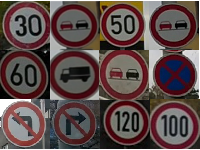
\includegraphics[width=1.0\linewidth,]{znacky.png}\\[1pt]
\caption{Ukázka vstupního datasetu pro trénování kaskádového klasifikátoru}
\label{fig:PositiveSigns}
\end{figure}

\subsection{Trénování kaskádového klasifikátoru}
\label{sec:Images}
Základem bylo vytvořit sadu pozitivních a negativních snímků pro natrénování kaskádového klasifikátoru. K tomuto účelu byl využit skript, který umožňuje detekci dopravních značek v barevném HSV modelu a následné vyhledávání tvarů pomocí Houghovy transformace (v nalezených konturách).

V případě nalezení objektu splňující definované požadavky je detekovaný objekt prohlášen za možnou značku a specifický výřez se uloží do složky pro pozitivní snímky. 

Naopak snímek, kde žádný takový objekt nebyl detekování je uložen do složky pro negativní vzorky.

Celkově bylo připraveno 400 pozitivních snímků zákazových značek a 1000 negativních z vytvořených zmiňovaným postupem. Jak vypadaly pozitivní smínky lze vidět na obrázku č. ~\ref{fig:PositiveSigns}. Tyto snímky byly použity pro vytvoření datového souboru pozitivních vzorků. Ten byl vytvářen aplikací \emph{opencv\_createsamples}%
	  \footnote{\url{http://docs.opencv.org/3.0-alpha/doc/user\_guide/ug\_traincascade.html\#training-data-preparation}}, která vytvářela vzorky o velikosti $50x50 px$, vzhledem k tomu že vstupní snímky obsahovaly pouze požadovanou oblast, tak nebylo příliš nutné zpracovávat soubor s anotacemi, ten obsahoval pouze seznam souborů s velikostí obrázků.

K trénování kaskádového klasifikátoru byla použita utilita \emph{opencv\_traincascade}%
\footnote{\url{http://docs.opencv.org/3.0-alpha/doc/user\_guide/ug\_traincascade.html\#cascade-training}}. Trénování bylo spuštěno s příznaky LBP, s počtem 10 iterací a parametrem \emph{\mbox{maxFalseAlarmRate}} s hodnotou 0.3.

\subsection{Klasifikace druhů značek}
S využitím funkčního kaskádového klasifikátoru bylo možné zpracovávat video záznamy a získávat soubory s detekovanými značkami. Tyto snímky následně byly rozděleny podle jednotlivých druhů a to zvlášť pro větší sadu určenou k trénování a menší určenou k testování klasifikace.

Metoda k-Nearest Neighbour funguje na principu hledání nejbližších sousedů v zadefinovaných příznacích. Ty je nutné si nejprve připravit. Jejich sestavení v tomto případě probíhá vytvořením binární reprezentace dopravní značky, což ilustruje obrázek č. ~\ref{fig:ClassificationTreshold}. Takováto binární reprezentace je poté převedena na jednodimenzionální pole, které je serializováno do souboru a oanotováno příslušným významem. Tento soubor si později načte klasifikátor pro kNN, který je dostupný v rámci knihovny OpenCV. Při klasifikaci je nutné klasifikovanou oblast upravit stejným způsobem jako při přípravě trénovacích dat, poté už stačí nechat určit klasifikátor do jaké třídy vzorek zařadí.

\begin{figure}[t]
\centering

\includegraphics[width=0.8\linewidth,]{classification_tresh.png}\\[1pt]
\caption{Vyprahovaná binární reprezentace dopravní značky pro klasifikaci druhu}
\label{fig:ClassificationTreshold}
\end{figure}

%--------------------------------------------------------
%--------------------------------------------------------
\subsection{Klasifikace rychlostního omezení}
\label{sec:Keywords}
Ze skupiny rychlostního omezení byly vybrány všechny snímky nad nimiž proběhla segmentace znaků a opět byly rozděleny do jednotlivých skupin podle významu jednotlivý znaků, tedy symbolů 0-9. Jednotlivé extrahované znaky lze vidět na obrázku č. ~\ref{fig:Symbols}. Následně bylo spuštěno automatické natrénování klasifikátoru z při\-pravené datové sady.

Klasifikace hodnoty nebyla vždy úplně přesná a proto bylo přistoupeno k porovnávání hodnot v rámci předešlých snímků a následné odfiltrování pravděpo\-dobně nerelevantních výsledků.

\begin{figure}[t]
\centering
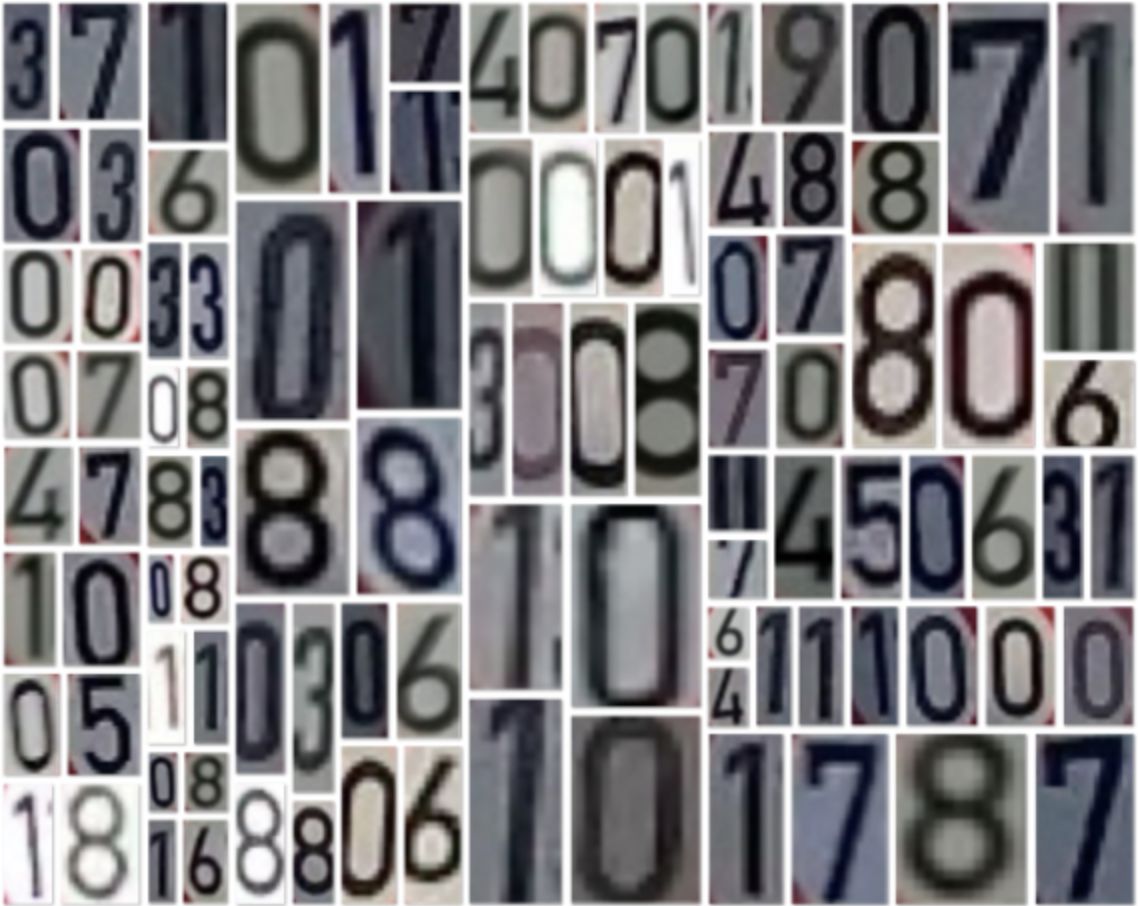
\includegraphics[width=0.8\linewidth,]{symboly.png}\\[1pt]
\caption{Dataset pro trénování klasifikace symbolů}
\label{fig:Symbols}
\end{figure}

\subsection{Trackování značky}
Vzhledem k tomu, že detekce ani klasifikace nebyly vždy stoprocentní, bylo nutné tyto nedostatky odstínit. V případě detekce k výpadku docházelo zejména u rozmazaných snímků. Ideálním způsobem se ukázalo sledování pozice dopravní značky a porovnávání klasifikovaných hodnot v předchozích snímcích.

Pokud na aktuálním snímku nebyla nalezena žádná značka, dojde ke kontrole přítomnosti značky na před\-chozím snímku. V případě, že je zde přítomné mini\-málně jedno dopravní značení, přistoupí se k vypočítání pravdě\-podobného umístění na aktuálním snímku, kde nedošlo k úspěšné detekci. To probíhá ze dvou předchozích známých pozic v rámci snímku.


\section{Experimenty}

\subsection{Úspěšnost detekce dopravních značek}
Pro vyhodnocení úspěšnosti detekce byly brány v potaz dva základní parametry a to \emph{True Positive} vypovídající o správné detekci a \emph{False Positive} vyjadřující chybnou detekci, kdy na snímku žádná značka není, ale klasifikátor označí nějakou oblast jako dopravní značku.

Pro vyhodnocení True Positive bylo využito při\-pravené testovací video, ze kterého byly vybrány vše\-chny snímky s dopravní značkou, celkově takových snímků bylo 520. Nad těmito snímky byl spuštěn kaskádový klasifikátor, který byl schopen dopravní značku detekovat celkově na 480 snímcích, procentuální úspěšnost je pak vyjádřena v tabulce č.  ~\ref{tab:SuccessTable}.

\begin{figure}[t]
\centering
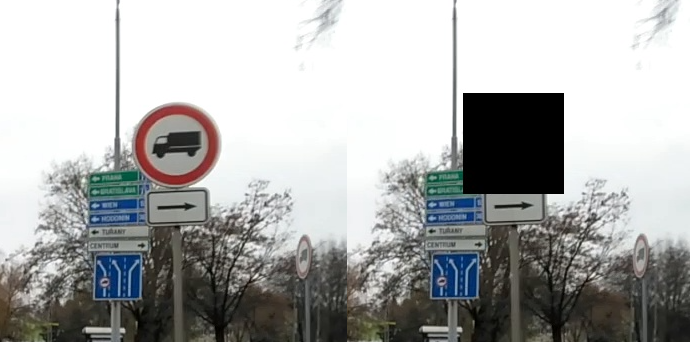
\includegraphics[width=1.0\linewidth,]{testdetekce.png}\\[1pt]
\caption{Zakrytí dopravních značek pro testování False Positive detekce}
  \label{fig:DetectionTest}
\end{figure}

V případě parametru \emph{False Positive} byly z testovacího vyextrahovány všechny snímky o celkovém počtu 1762. Na snímcích, kde se nacházely dopravní značky došlo k zakrytí těchto oblastí jak je vidět na obrázku č. ~\ref{fig:DetectionTest}. Kaskádový klasifikátor byl opět spuštěn nad těmito snímky a výsledkem je velmi nízké číslo nechtěných detekcí s hodnotou $0.45 \%$ viz. tabulka č. ~\ref{tab:SuccessTable}. Toto číslo lze navíc snadno ještě snížit, díky tomu, že nad detekovanými oblastmi probíhá další klasifikace.

\begin{table}[h]
	\vskip6pt
	\caption{Úspěšnost detekce}
	\centering
	\begin{tabular}{llr}
		\toprule
		True Positive & $92.3 \%$ \\
		False Positive & $0.45 \%$ \\
		\bottomrule
	\end{tabular}
	\label{tab:SuccessTable}
\end{table}

\subsection{Úspěšnost klasifikace druhu}
Testování rozlišení klasifikace druhu dopravní značky probíhalo na datové skupině zahrnující pět druhů značek po pěti vzorcích. Sada pro trénování obsahovalo vzorku 50. Dosažená úspěšnost nad testovacími daty dosahovala 87 \%.

\subsection{Zpracování jednoho záznamu}

Tento experiment ukazuje proces zpracování jednoho záznamu. Záznam byl pořízen běžným mobilní telefonem s operačním systém Android pomocí aplikace AutoBoy Dash Cam - BlackBox \cite{autoboy}. Pořízený záznam má rozlišení 1280x720 px s frekvencí 30 snímků za sekundu. Celková délka záznamu činí  přesně pět minut a velikost videosouboru je  451 MB.  K záznamu byl vygenerován  standardní SRT soubor. Ten obsahuje  bloky informací, kde  vždy jeden záznam  reprezentuje čas platnosti, aktuální rychlost, GPS souřadnice a adresu místa pořízení. Tyto informace jsou vždy po jedné sekundě, což dostačuje k určení pozice.

Skript byl spuštěn se zadáním parametrů pořízeného videa a  přiloženého SRT souboru. Celý proces zpracování trval 199 s,  rychlost zpracování tedy odpovídá přibližně 45 snímků za sekundu.

Výsledkem je CSV soubor, který obsahuje celkově sedm řádků,  kdy se na každém řádku nachází hodnota rychlostního omezení, a zeměpisná šířka a délka. Úspěšnost detekce a klasifikace je v tomto případě 100\%. Vytvořený soubor byl nahrán do webové služby Google Fusion Tables. Ta umožňuje z  importované tabulky vykreslit  interaktivní mapu jejíž náhled  lze vidět obrázku č. ~\ref{fig:RecordPreview}.


\begin{figure}[t!]
\centering
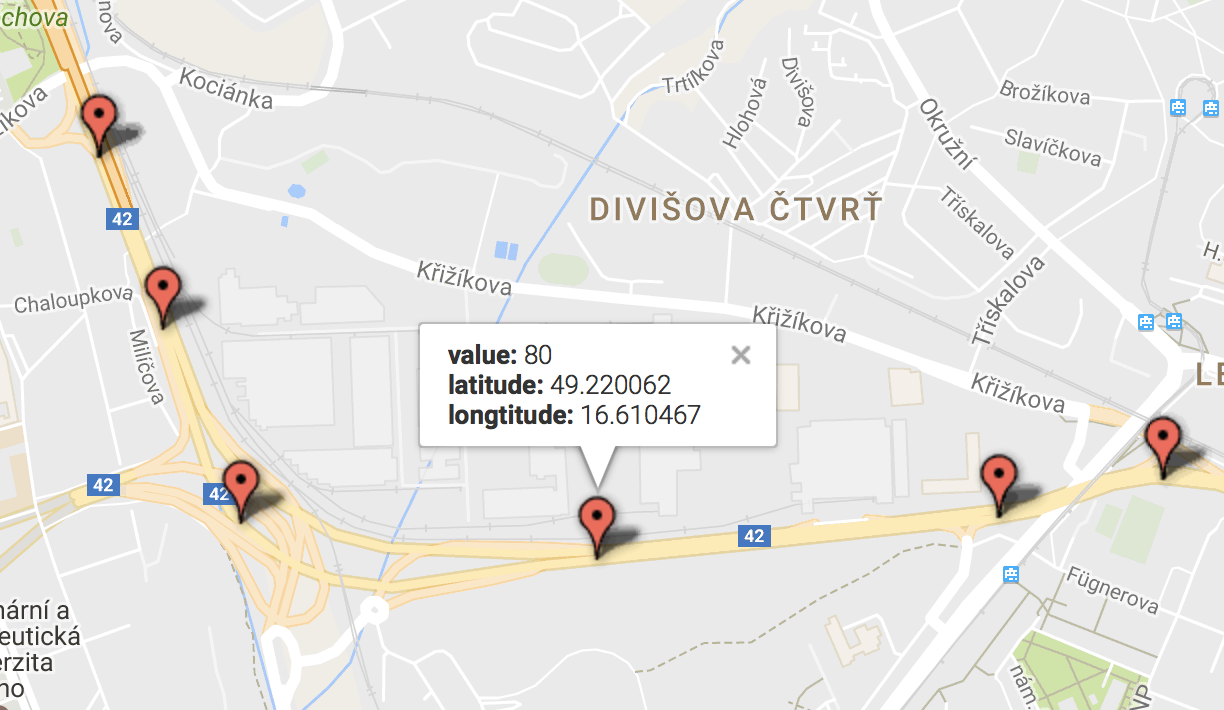
\includegraphics[width=1.0\linewidth,]{mapa.png}\\[1pt]
\caption{Ukázka vizualizace jednoho zpracovaného videozáznamu}
  \label{fig:RecordPreview}
\end{figure}

%--------------------------------------------------------
%--------------------------------------------------------
%--------------------------------------------------------
%--------------------------------------------------------


%--------------------------------------------------------
%--------------------------------------------------------
%--------------------------------------------------------
%--------------------------------------------------------
\section{Shrnutí}
\label{sec:Conclusions}

V práci byl prezentován postup analýzy záznamu automobilu vedoucí ke zmapování dopravního značení. Výsledkem je navrhnutý a implementovaný proces celé analýzy.

Práce ukazuje jak lze využít kaskádový klasifikátor pro detekci dopravních značek a jak je možné vytvořit datovou sadu pro trénování.  Dále je přednesena možnost jak realizovat klasifikaci dopravního značení metodou kNN a to nejen pro klasifikaci typu, ale i klasifikaci konkrétní hodnoty.

Všechny zdrojové kódy jsou zveřejněny ve veřejném repozitáři služby \emph{GitHub}%
	  \footnote{\url{https://github.com/jankaderabek/dashcam-analyzer}} . To dává možnost komukoliv na ně nahlédnout a využít je jako inspiraci pro vlastní práci, případně poskytuje možnost navrhnout možná vylepšení současné práce. 

Hlavním cílem budoucí práce je pokrýt všechny dopravní značky a získat tak větší množství dat pro další agregaci.

S tím souvisí nabídnutí možnosti veřejnosti jak pomoci se shromažďováním dat. Ideálním řešením se jeví webová aplikace,  která by byla schopna  zaznamenat zpracovaná data ze záznamů. 

Následně by bylo možné  realizovat různé analýzy nad získanými daty a nabídnout například přehled dopravního značení v širším měřítku.


\section*{Poděkování}
Za veškerou pomoc během bakalářské práce, v rámci které vznikl i tento článek, bych chtěl poděkovat svému vedoucímu Ing. Jakubovi Špaňhelovi.

%--------------------------------------------------------
%--------------------------------------------------------
%--------------------------------------------------------
%	REFERENCE LIST
%--------------------------------------------------------
%--------------------------------------------------------
\phantomsection
\bibliographystyle{unsrt}
\bibliography{2017-ExcelFIT-OnBoardCameraAnalysis-bib}


%--------------------------------------------------------
%--------------------------------------------------------
%--------------------------------------------------------
\end{document}